\documentclass[12pt,-letter paper]{article}
\usepackage{siunitx}
\usepackage{setspace}
\usepackage{gensymb}
\usepackage{xcolor}
\usepackage{caption}
%\usepackage{subcaption}
\doublespacing
\singlespacing
\usepackage[none]{hyphenat}
\usepackage{amssymb}
\usepackage{relsize}
\usepackage[cmex10]{amsmath}
\usepackage{mathtools}
\usepackage{amsmath}
\usepackage{commath}
\usepackage{amsthm}
\interdisplaylinepenalty=2500
%\savesymbol{iint}
\usepackage{txfonts}
%\restoresymbol{TXF}{iint}
\usepackage{wasysym}
\usepackage{amsthm}
\usepackage{mathrsfs}
\usepackage{txfonts}
\let\vec\mathbf{}
\usepackage{stfloats}
\usepackage{float}
\usepackage{hyperref}
\usepackage{cite}
\usepackage{cases}
\usepackage{subfig}
%\usepackage{xtab}
\usepackage{longtable}
\usepackage{multirow}
%\usepackage{algorithm}
\usepackage{amssymb}
%\usepackage{algpseudocode}
\usepackage{enumitem}
\usepackage{mathtools}
%\usepackage{eenrc}
%\usepackage[framemethod=tikz]{mdframed}
\usepackage{listings}
%\usepackage{listings}
\usepackage[latin1]{inputenc}
%%\usepackage{color}{   
%%\usepackage{lscape}
\usepackage{textcomp}
\usepackage{titling}
\usepackage{hyperref}
%\usepackage{fulbigskip}   
\usepackage{tikz}
\usepackage{graphicx}
%\usepackage[left=1in, right=2in, top=1in, bottom=1in]{geometry}

\let\vec\mathbf{}
\usepackage{enumitem}
\usepackage{graphicx}
\usepackage{siunitx}
\let\vec\mathbf{}
\usepackage{enumitem}
\usepackage{graphicx}
\usepackage{enumitem}
\usepackage{tfrupee}
\usepackage{amsmath}
\usepackage{amssymb}
\usepackage{tfrupee}
\DeclareMathOperator*{\Res}{Res}
\newtheorem{theorem}{Theorem}[section]
\newtheorem{problem}{Problem}
\newtheorem{proposition}{Proposition}[section]
\newtheorem{lemma}{Lemma}[section]
\newtheorem{corollary}[theorem]{Corollary}
\newtheorem{example}{Example}[section]
\newtheorem{definition}[problem]{Definition}
\newcommand{\BEQA}{\begin{eqnarray}}
\newcommand{\EEQA}{\end{eqnarray}}
\newcommand{\define}{\stackrel{\triangle}{=}}
\theoremstyle{remark}
\newtheorem{rem}{Remark}

\renewcommand{\thefigure}{\theenumi}
\renewcommand{\thetable}{\theenumi}
\providecommand{\pr}[1]{\ensuremath{\Pr\left(#1\right)}}
\providecommand{\prt}[2]{\ensuremath{p_{#1}^{\left(#2\right)} }}        % own macro for this question
\providecommand{\qfunc}[1]{\ensuremath{Q\left(#1\right)}}
\providecommand{\sbrak}[1]{\ensuremath{{}\left[#1\right]}}
\providecommand{\lsbrak}[1]{\ensuremath{{}\left[#1\right.}}
\providecommand{\rsbrak}[1]{\ensuremath{{}\left.#1\right]}}
\providecommand{\brak}[1]{\ensuremath{\left(#1\right)}}
\providecommand{\lbrak}[1]{\ensuremath{\left(#1\right.}}
\providecommand{\rbrak}[1]{\ensuremath{\left.#1\right)}}
\providecommand{\cbrak}[1]{\ensuremath{\left\{#1\right\}}}
\providecommand{\lcbrak}[1]{\ensuremath{\left\{#1\right.}}
\providecommand{\rcbrak}[1]{\ensuremath{\left.#1\right\}}}
\newcommand{\sgn}{\mathop{\mathrm{sgn}}}
\providecommand{\abs}[1]{\left\vert#1\right\vert}
\providecommand{\res}[1]{\Res\displaylimits_{#1}} 
\providecommand{\norm}[1]{\left\lVert#1\right\rVert}
%\providecommand{\norm}[1]{\lVert#1\rVert}
\providecommand{\mtx}[1]{\mathbf{#1}}
\providecommand{\mean}[1]{E\left[ #1 \right]}
\providecommand{\cond}[2]{#1\middle|#2}
\providecommand{\fourier}{\overset{\mathcal{F}}{ \rightleftharpoons}}
%\providecommand{\hilbert}{\overset{\mathcal{H}}{ \rightleftharpoons}}
%\providecommand{\system}{\overset{\mathcal{H}}{ \longleftrightarrow}}
	%\newcommand{\solution}[2]{\textbf{Solution:}{#1}}
\newcommand{\solution}{\noindent \textbf{Solution: }}
\newcommand{\cosec}{\,\text{cosec}\,}
\providecommand{\dec}[2]{\ensuremath{\overset{#1}{\underset{#2}{\gtrless}}}}
\newcommand{\myvec}[1]{\ensuremath{\begin{pmatrix}#1\end{pmatrix}}}
\newcommand{\mydet}[1]{\ensuremath{\begin{vmatrix}#1\end{vmatrix}}}
\providecommand{\rank}{\text{rank}}
\providecommand{\pr}[1]{\ensuremath{\Pr\left(#1\right)}}
\providecommand{\qfunc}[1]{\ensuremath{Q\left(#1\right)}}
	\newcommand*{\permcomb}[4][0mu]{{{}^{#3}\mkern#1#2_{#4}}}
\newcommand*{\perm}[1][-3mu]{\permcomb[#1]{P}}
\newcommand*{\comb}[1][-1mu]{\permcomb[#1]{C}}
\providecommand{\qfunc}[1]{\ensuremath{Q\left(#1\right)}}
\providecommand{\gauss}[2]{\mathcal{N}\ensuremath{\left(#1,#2\right)}}
\providecommand{\diff}[2]{\ensuremath{\dfrac{d{#1}}{d{#2}}}}
\providecommand{\myceil}[1]{\left \lceil #1 \right \rceil }
\newcommand{\sinc}{\,\text{sinc}\,}
\newcommand{\rect}{\,\text{rect}\,}
\newcommand{\E}{\mathbb{E}}
\newcommand{\Var}{\mathrm{Var}}


\begin{document}
\vspace{3cm}

\title{Assignment}
\author{FWC22244 - Sarvesh K}
\maketitle
\begin{enumerate}
      \section{Vectors}
\item  Prove that the points $\myvec{3,0}, \myvec{6, 4}$ and $\myvec{-1, 3}$ are the vertices of a right angled isosceles triangle.\\
\item  If the point $P\myvec{x, y}$ is equidistant from the points $A\myvec{a+b, b-a}$ and $B\myvec{a-b, a+b}$. Prove that $bx=ay$.\\
\item In fig \ref{figure_1}, the vertices of $\triangle ABC$ are $A\myvec{4, 6}, B\myvec{1, 5}$and $C\myvec{7, 2}$. A line-segment $DE$ is drawn to intersect the sides $AB$ and $AC$ at $D$ and $E$ respectively such that $\dfrac{AD}{AB}$ = $\dfrac{AE}{AC}$ = $\dfrac{1}{3}$ . Calculate the area of $ \triangle ADE$ and compare it with area of $ \triangle ABC$.\\
	\begin{figure}[H]
      \centering
      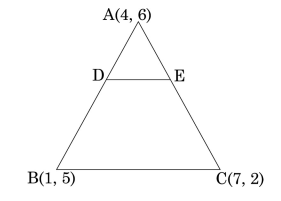
\includegraphics[width=5cm]{figs/8.png}
     \caption{}
      \label{figure_1}
\end{figure} 
\item  Let $P$ and $Q$ be the points of trisection of the line segment joining the points $A\myvec{2,-2}$ and $B\myvec{-7, 4}$ such that $P$ is nearer to $A$. Find the coordinates of $P$ and $Q$.\\

\section{Circles}
\item In Fig \ref{figure_2}, $PQ$ is a tangent at point $C$ to a circle with centre $O$. If $AB$ is a diameter and $\angle CAB = 30\degree $, Find $\angle PCA$.\\
\begin{figure}[H]
\centering
	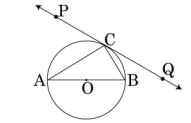
\includegraphics[width=5cm]{figs/1.png}
	\caption{}
\label{figure_2}
\end{figure} 
\item  In Fig \ref{figure_3}, a quadrilateral $ABCD$ is drawn to circumscribe a circle, with centre $O$, in such a way that the sides $AB, BC, CD$ and $DA$ touch the circle at the points $P, Q, R$ and $S$ respectively. Prove that $ AB + CD= BC + DA $.\\
	\begin{figure}[H]
\centering
      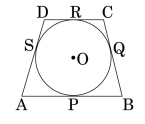
\includegraphics[width=5cm]{figs/2.png}
      \caption{}
      \label{figure_3}
\end{figure} 
\item  In Fig \ref{figure_4}, from an external point $P$, two tangents $PT$ and $PS$ are drawn to a circle with centre $O$ and radius $r$. If $OP = 2r$, show that $\angle OTS = \angle OST= 30\degree$.
\begin{figure}[H]
\centering
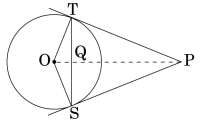
\includegraphics[width=5cm]{figs/3.png}
\caption{}
      \label{figure_4}
   \end{figure} 
 \item  In fig \ref{figure_5}, $O$ is the centre of a circle such that diameter $AB = 13$ cm and $AC = 12$ cm. $BC$ is joined. Find the area of the shaded region. (Take $\pi = 3.14$)\\

	\begin{figure}[H]
      \centering
      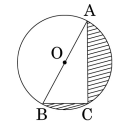
\includegraphics[width=5cm]{figs/4.png}
      \caption{}
      \label{figure_5}
\end{figure} 
\item In Fig \ref{figure_6} , two equal circles, with centres $O$ and $O^\prime$, touch each other at $X$.$OO\prime$ produced meets the circle with centre $O^\prime$ at $A$. $AC$ is tangent to the circle with centre $O$, at the point $C$. $O^\prime D$ is perpendicular to $AC$. Find the value of $\dfrac{DO^\prime}{CO^\prime}$.\\
	\begin{figure}[H]
      \centering
      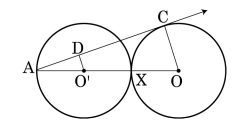
\includegraphics[width=5cm]{figs/7.png}
      \caption{}
      \label{figure_6}
   \end{figure} 
 
\item Prove that the lengths of the tangents drawn from an external point to a circle are equal.\\  

\section{Probability}
\item A card is drawn at random from a well shuffled pack of $52$ playing cards. Find the probability of getting neither a red card nor a queen.\\
\item There are $100$ cards in a bag on which numbers from $1$ to $100$ are written. A card is taken out from the bag at random. Find the probability that the number on the selected card 
\begin{enumerate}[label=(\roman*)]
\item is divisible by $9$ and is a perfect square 
\item is a prime number greater than $80$
\end{enumerate}
\item A number $x$ is selected at random from the numbers $1, 2, 3$ and $4$. Another number $y$ is selected at random from the numbers $1, 4, 9$ and $16$. Find the probability that product of $x$ and $y$ is less than $16$.\\
\item From a pack of $52$ playing cards, Jacks, Queens and Kings of red colour are removed. From the remaining, a card is drawn at random. Find the probability that drawn card is :
\begin{enumerate}[label=(\roman*)]
\item a black King 
\item a card of red colour 
\item a card of black colour
\end{enumerate}
\item  Three different coins are tossed together. Find the probability of getting 
\begin{enumerate}[label=(\roman*)]
\item exactly two heads 
\item at least two heads 
\item at least two tails.
\end{enumerate}

\section{Algebra}
\item If $-5$ is a root of the quadratic equation $2x^2+px-15=0$ and the quadratic equation $p\brak{x^2+x}+k=0 $ has equal roots, find the value of $k$. \\
\item Solve for $x$ : 
\begin{align*}\sqrt{2x+9} + x = 13\end{align*}
\item Solve for $x$ :
\begin{align*}\sqrt{6x+7}-\brak{2x-7}= 0\end{align*}
\item If the roots of the quadratic equation $\brak{a-b}x^2+\brak{b-c}x+\brak{c-a}=0$ are equal,prove that $2a=b+c$.\\
\item  Solve for $ x$ :  \begin{align*} \dfrac{1}{\brak{x-1}\brak{x-2}}  +  \dfrac{1}{\brak{x-2}\brak{x-3}}  =  \dfrac{2}{3} , x \neq 1,2,3\end{align*}
\item  Solve for $ x$ :  \begin{align*} \dfrac{1}{x+1}  + \dfrac{2}{x+2}  = \dfrac{4}{x+4} , x \neq -1,-2,-4 \end{align*} 
\item A motor boat whose speed is $24$ km/h in still water takes 1 hour more to go $32$ km upstream than to return downstream to the same spot. Find the speed of the stream.\\
\item Three consecutive natural numbers are such that the square of the middle number exceeds the difference of the squares of the other two by $60$. Find the numbers.\\
\item Two pipes running together can fill a tank in $11\dfrac{1}{5}$ minutes. If one pipe takes $5$ minutes more than the other to fill the tank separately, find the time in which each pipe would fill the tank separately.\\

\section{Geometry}
\item A ladder, leaning against a wall, makes an angle of $60 \degree$ with the horizontal.If the foot of the ladder is $2.5$ m away from the wall, find the length of the ladder.\\
\item  In \ref{figure_7}, a tent is in the shape of a cylinder surmounted by a conical top of same diameter. If the height and diameter of cylindrical part are $2.1$ m and $3$ m respectively and the slant height of conical part is $2.8$ m, find the cost of canvas needed to make the tent if the canvas is available at the rate of \rupee $500$/sq.metre.$\brak{\text{Use } \pi = \dfrac{22}{7}}$\\
	\begin{figure}[H]
      \centering
      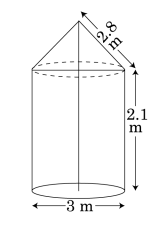
\includegraphics[width=5cm]{figs/5.png}
      \caption{}
      \label{figure_7}
\end{figure} 
\item  In \ref{figure_8}, find the area of the shaded region, enclosed between two concentric circles of radii $7$ cm and $14$ cm where $\angle AOC = 40\degree$ $\brak{\text{Use }\pi =\dfrac{22}{7}}$.
	\begin{figure}[H]
      \centering
      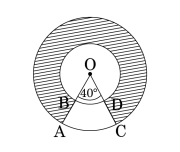
\includegraphics[width=5cm]{figs/6.png}
      \caption{}
      \label{figure_8}
\end{figure} 
\item  A conical vessel, with base radius $5$ cm and height $24$ cm, is full of water. This water is emptied into a cylindrical vessel of base radius $10$ cm. Find the height to which the water will rise in the cylindrical vessel. $\brak{\text{Use } \pi  = \dfrac{22}{7}}$\\
\item  A sphere of diameter $12$ cm, is dropped in a right circular cylindrical vessel, partly filled with water. If a sphere is completely submerged in water, the water level in the cylindrical vessel rises by $ 3 \dfrac{5}{9}$cm. Find the diameter of the cylindrical vessel.\\  
\item  Due to heavy floods in a state, thousands were rendered homeless. $50$ schools collectively offered to the state government to provide place and the canvas for $1500$ tents to be fixed by the government and decided to share the whole expenditure equally. The lower part of each tent is cylindrical of base radius $2.8$ m and height $3.5$ m, with conical upper part of same base radius but of height $2.1$ m. If the canvas used to make the tents costs \rupee~120 per sq.m, find the amount shared by each school to set up the tents. What value is generated by the above problem ? (Use $ \pi = \dfrac{22}{7} ) $\\
\item  A man standing on the deck of a ship, which is $10$ m above water level, observes the angle of elevation of the top of a hill as $ 60\degree $ and the angle of depression of the base of hill as $ 30 \degree $. Find the distance of the hill from the ship and the height of the hill.\\
\item The angle of elevation of the top $Q$ of a vertical tower $PQ$ from a point $X$ on the ground is $ 60\degree $. From a point $Y$, $40$ m vertically above $X$, the angle of elevation of the top $Q$ of tower is $ 45 \degree $. Find the height of the tower $PQ$ and the distance $PX$. $\brak{\text{Use }\sqrt{3} = 1.73}$\\
\item A rectangular park is to be designed whose breadth is $3$ m less than its length.Its area is to be $4$ square metres more than the area of a park that has already been made in the shape of an isosceles triangle with its base as the breadth of the rectangular park and of altitude $12$ m. Find the length and breadth of the rectangular park.\\
\item In Fig  \ref{figure_9} , is shown a sector $OAP$ of a circle with centre $O$, containing $\angle \theta$. $AB$ is perpendicular to the radius $OA$ and meets $OP$ produced at $B$. Prove that the perimeter of shaded region is $r\sbrak{\tan \theta + \sec \theta + \dfrac{\pi \theta}{180}-1}$ \\

	\begin{figure}[H]
      \centering
      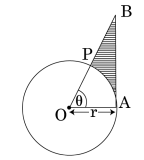
\includegraphics[width=5cm]{figs/9.png}
     \caption{}
     \label{figure_9}
\end{figure} 

\section{Discrete}
\item For what value of $k$ will $k+9, 2k-1$ and $2k+7$ are the consecutive terms of an A.P ?\\
\item  The $4$th term of an A.P. is zero. Prove that the $25$th term of the A.P. is three times its $11$th term.\\
\item  If the ratio of the sum of first $n$ terms of two A.P's is $\brak{7n + 1} : \brak{4n + 27}$, find the ratio of their $m$ th terms.\\
\item The sums of first $n$ terms of three arithmetic progressions are $S_1, S_2$ and $S_3$ respectively. The first term of each A.P. is $1$ and their common differences are $1, 2$ and $3$ respectively. Prove that $S_1+S_3=S_2$.\\
\item The digits of a positive number of three digits are in A.P. and their sum is $15$.The number obtained by reversing the digits is $594$ less than the original number. Find the number.\\
\item The houses in a row are numbered consecutively from $1$ to $49$. Show that there exists a value of $X$ such that sum of numbers of houses preceeding the house numbered $X$ is equal to sum of the numbers of houses following $X$.\\

\section{Constructions}    
\item Draw a circle of radius $4$ cm. Draw two tangents to the circle inclined at an angle of $ 60 \degree $ to each other.\\
\item Draw a triangle with sides $5$ cm, $6$ cm and $7$ cm. Then draw another triangle whose sides are $\dfrac{4}{5}$ of the corresponding sides of first triangle.\\
\item Draw an isosceles $\triangle ABC$ in which $BC=5.5 cm$ and altitude $AL=5.3 cm$. Then construct another triangle whose sides are $\dfrac{3}{4}$ of the corresponding sides of $\triangle ABC$.\\
\end{enumerate}
\end{document}
